\documentclass[12pt,a4paper]{article}
\usepackage{graphicx}
\usepackage{wrapfig}
\usepackage{textcomp}
\usepackage{multicol}

\title{Praktikum Physik - Bestimmung von $\frac{c_p}{c_V}$}
\author{Simon Marti, Patricia Schwab, Mirco Kocher}
\date{04.05.2012}


\begin{document}
\maketitle

\section*{Ziel}
Bestimmung der Gr\"osse $\kappa$ f\"ur die Gase CO$_2$, Ar und N$_2$. Die Werte sollen danach mit den Literaturangaben verglichen werden.


\section*{Motivation}
Anhand dieses Experiments mit drei allt\"aglichen Gasen sollen einige thermodynamische Grundlagen vertieft werden.


\section*{Theorie}
Die Gr\"osse $\kappa$ ist definiert als Verh\"altnis der isobaren W\"armekapazit\"at $c_p$ zur isochoren W\"armekapazit\"at $c_V$
\begin{equation}
\kappa = \frac{c_p}{c_V}
\end{equation}
Die Tabellenwerte f\"ur $\kappa$ von Kohlendioxid CO$_2$, Stickstoff N$_2$ und Argon Ar sind
\begin{eqnarray}
\kappa_{CO_2} & \approx & 1.30 \\
\kappa_{N_2} & \approx & 1.404 \\
\kappa_{Ar} & \approx & 1.670 \
\end{eqnarray}
Mit dem Aussendruck $p_a$, der Gravitationskraft $g$, der Masse der Kugel $m$ und der Querschnittsfl\"ache $A$ des Rohres ist der Druck $p_0$ definiert als
\begin{eqnarray}
p_0 & = & p_a + \frac{mg}{A} \label{eq:p}\\
p_a & = & (94050 \pm 50) \mbox{Pa}
\end{eqnarray}
Die Schwingung der Kugel l\"asst sich folgendermassen beschreiben
\begin{eqnarray}
\omega & = & \frac{2\pi}{T} = \sqrt{\frac{\kappa p_0 A^2}{m V_0}}
\end{eqnarray}
Dadurch erh\"alt man $\kappa$ in Abh\"angigkeit von $T$
\begin{eqnarray}
\Rightarrow \kappa & = & \frac{4\pi ^2 m V_0}{p_0 A^2 T^2}\label{eq:k}
\end{eqnarray}

\section*{Aufbau und Ablauf}
\begin{wrapfigure}[20]{r}{9cm}
\vspace{-30pt}
\centering
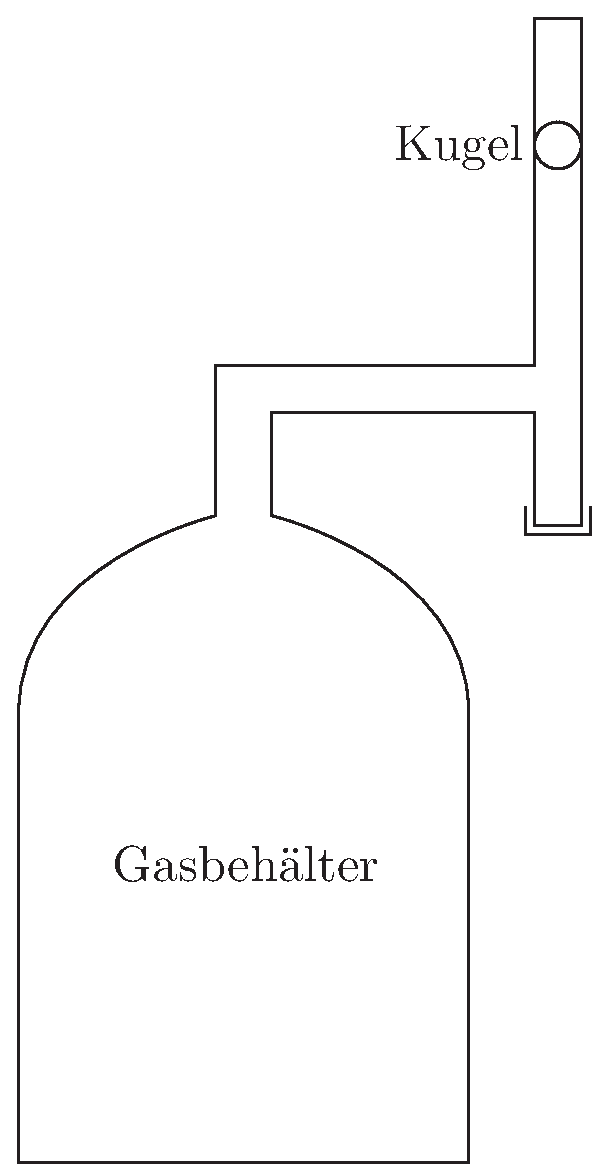
\includegraphics[width=6cm]{illustration.pdf}
\end{wrapfigure}
Ein geschlossener und mit Gas gef\"ullter Glasbeh\"alter ist mit einem vertikal ausgerichteten Glasrohr verbunden welches unten verschlossen werden kann. Eine Metallkugel mit gleichem Durchmesser wie das Rohr wird nun von oben in dieses fallen gelassen und die Periode der resultierenden Schwingung mithilfe einer Stoppuhr bestimmt. Gemessen wurden jeweils 5 Perioden von Mirco.


\section*{Rohdaten}
\begin{eqnarray*}
d & = & 16.0\mbox{mm} \\
m & = & (17.0 \pm 0.1) \mbox{g}
\end{eqnarray*} 
\subsection*{Volumen}
Das Volumen des Glasbeh\"alters ist mit $V_{Flasche}$ = (5616 $\pm $ 5) cm$^3$. Dazu kommt durchschnittlich 39cm Glasrohr was $\overline{V}_{Rohr}$ = 78.414 cm$^3$ entspricht.
\[ \Rightarrow \overline{V} = V_{Flasche} + \overline{V}_{Rohr} = 0.005694\mbox{m}^3 \]

\begin{multicols}{3}
\subsection*{CO$_2$}
\begin{tabular}{|r|r|}
\hline
$i$&5$T$ [s]\\
\hline
1&4.37 \\
2&4.27 \\
3&4.48 \\
4&4.47 \\
5&4.30 \\
\hline
\end{tabular}

\subsection*{N$_2$}
\begin{tabular}{|r|r|}
\hline
$i$&5$T$ [s]\\
\hline
1&4.26 \\
2&4.27 \\
3&4.31 \\
4&4.26 \\
5&4.16 \\
\hline
\end{tabular}

\subsection*{Ar}
\begin{tabular}{|r|r|}
\hline
$i$&5$T$ [s]\\
\hline
1&3.86 \\
2&3.90 \\
3&3.83 \\
4&3.98 \\
5&3.79 \\
\hline
\end{tabular}
\end{multicols}

\section*{Auswertung}
\subsection*{CO$_2$}
Periode
\[ \overline{T} = 0.8756\mbox{s} \]
$\kappa$ nach Formel (\ref{eq:k}):
\[ \kappa_{CO_2} = 1.29961 \]

\subsection*{N$_2$}
Periode
\[ \overline{T} = 0.8504\mbox{s} \]
$\kappa$ nach Formel (\ref{eq:k}):
\[ \kappa_{N_2} = 1.37778 \]

\subsection*{Ar}
Periode
\[ \overline{T} = 0.7744\mbox{s} \]
$\kappa$ nach Formel (\ref{eq:k}):
\[ \kappa_{Ar} = 1.66148 \]

\newpage
\section*{Fehlerrechnung}
Formel (\ref{eq:k}) h\"angt unter Ber\"ucksichtigung von (\ref{eq:p}) von f\"unf Gr\"ossen ab. (Als $T$ wurde $\overline{T}_{Ar}$ eingesetzt.)
\begin{eqnarray*}
\frac{\partial \kappa}{\partial T} & = & -4.291\\
\frac{\partial \kappa}{\partial V} & = & 291.77\\
\frac{\partial \kappa}{\partial m} & = & 96.880\\
\frac{\partial \kappa}{\partial r} & = & -827.11\\
\frac{\partial \kappa}{\partial p_a} & = & -0.0017512\\
\end{eqnarray*}

\noindent
Aufgrund dieser Werte k\"onnen wir den Fehler $s_{p_a}$ vernachl\"assigen, den unbekannten Fehler $s_r$ sollten wir aber zumindest absch\"atzen.

\begin{eqnarray*}
s_T & = & 0.5 \mbox{s}\hspace{2pt}/\hspace{2pt}5\hspace{2pt}\mbox{Perioden}\hspace{2pt}/\hspace{2pt}5\hspace{2pt}\mbox{Messungen} = 0.02 \mbox{s}\\
s_V & = & 10^{-5} \mbox{m}^3\\
s_m & = & 10^{-4} \mbox{kg}\\
s_r & = & 2\cdot 10^{-5} \mbox{m}\\
\end{eqnarray*}

\begin{eqnarray*}
s_\kappa & = & \left( \frac{\partial \kappa}{\partial T}\right) ^2\cdot s_T^2 + \left( \frac{\partial \kappa}{\partial V}\right) ^2\cdot s_V^2 + \left( \frac{\partial \kappa}{\partial m}\right) ^2\cdot s_m^2 + \left( \frac{\partial \kappa}{\partial r}\right) ^2\cdot s_r^2\\
& = & 0.00774
\end{eqnarray*}

\section*{Diskussion}
Die Abweichung zu den Tabellenwerten betr\"agt etwa 0.00039 f\"ur CO$_2$, 0.0085 f\"ur Ar und 0.026 f\"ur N$_2$. Bis auf die Messung mit Stickstoff sind diese Differenzen kleiner als der berechnete Fehler. Die etwas gr\"ossere Abwei\-chung f\"ur Stickstoff ist h\"ochstwahrscheinlich auf eine schlechte Zeitmessung zur\"uckzuf\"uhren da die anderen Werte mit gleichen Bedingungen relativ genau berechnet werden konnten. Eine andere m\"ogliche Fehlerquelle w\"are ein unreines Gasgemisch im Glasbeh\"alter.

\end{document}